\documentclass{article}\usepackage[]{graphicx}\usepackage[]{xcolor}
% maxwidth is the original width if it is less than linewidth
% otherwise use linewidth (to make sure the graphics do not exceed the margin)
\makeatletter
\def\maxwidth{ %
  \ifdim\Gin@nat@width>\linewidth
    \linewidth
  \else
    \Gin@nat@width
  \fi
}
\makeatother

\definecolor{fgcolor}{rgb}{0.345, 0.345, 0.345}
\newcommand{\hlnum}[1]{\textcolor[rgb]{0.686,0.059,0.569}{#1}}%
\newcommand{\hlstr}[1]{\textcolor[rgb]{0.192,0.494,0.8}{#1}}%
\newcommand{\hlcom}[1]{\textcolor[rgb]{0.678,0.584,0.686}{\textit{#1}}}%
\newcommand{\hlopt}[1]{\textcolor[rgb]{0,0,0}{#1}}%
\newcommand{\hlstd}[1]{\textcolor[rgb]{0.345,0.345,0.345}{#1}}%
\newcommand{\hlkwa}[1]{\textcolor[rgb]{0.161,0.373,0.58}{\textbf{#1}}}%
\newcommand{\hlkwb}[1]{\textcolor[rgb]{0.69,0.353,0.396}{#1}}%
\newcommand{\hlkwc}[1]{\textcolor[rgb]{0.333,0.667,0.333}{#1}}%
\newcommand{\hlkwd}[1]{\textcolor[rgb]{0.737,0.353,0.396}{\textbf{#1}}}%
\let\hlipl\hlkwb

\usepackage{framed}
\makeatletter
\newenvironment{kframe}{%
 \def\at@end@of@kframe{}%
 \ifinner\ifhmode%
  \def\at@end@of@kframe{\end{minipage}}%
  \begin{minipage}{\columnwidth}%
 \fi\fi%
 \def\FrameCommand##1{\hskip\@totalleftmargin \hskip-\fboxsep
 \colorbox{shadecolor}{##1}\hskip-\fboxsep
     % There is no \\@totalrightmargin, so:
     \hskip-\linewidth \hskip-\@totalleftmargin \hskip\columnwidth}%
 \MakeFramed {\advance\hsize-\width
   \@totalleftmargin\z@ \linewidth\hsize
   \@setminipage}}%
 {\par\unskip\endMakeFramed%
 \at@end@of@kframe}
\makeatother

\definecolor{shadecolor}{rgb}{.97, .97, .97}
\definecolor{messagecolor}{rgb}{0, 0, 0}
\definecolor{warningcolor}{rgb}{1, 0, 1}
\definecolor{errorcolor}{rgb}{1, 0, 0}
\newenvironment{knitrout}{}{} % an empty environment to be redefined in TeX

\usepackage{alltt}
\usepackage[T1]{fontenc}                
\usepackage[utf8]{inputenc}             
\usepackage[english]{babel}
\newcommand{\ped}[1]{$_{#1}$}
\usepackage{tikz}
  \usetikzlibrary{shapes,arrows,fit,calc,positioning}
  \tikzset{box/.style={draw, diamond, thick, text centered, minimum height=0.5cm, minimum width=1cm}}
  \tikzset{line/.style={draw, thick, -latex'}}
\IfFileExists{upquote.sty}{\usepackage{upquote}}{}
\begin{document}
    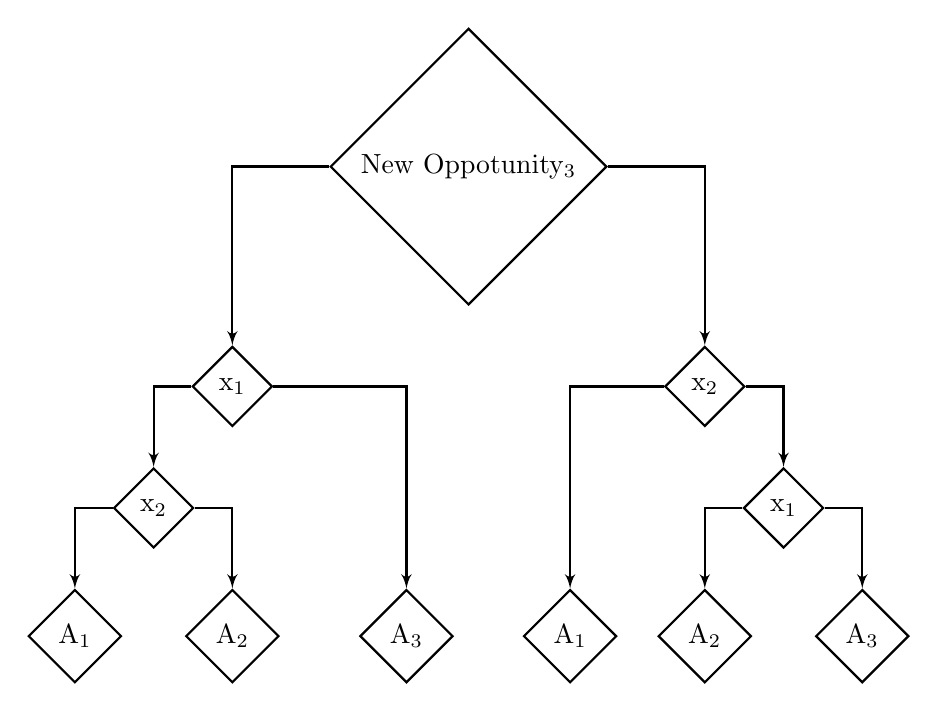
\begin{tikzpicture}[auto]
        \node [box]                                    (x3)      {New Oppotunity\ped{3}};
        \node [box, below=0.5cm of x3, xshift=-3cm]    (x1sx)    {x\ped{1}};
        \node [box, below=0.5cm of x3, xshift=3cm]     (x2dx)    {x\ped{2}};
        \node [box, below=0.5cm of x1sx, xshift=-1cm]  (x2sx)    {x\ped{2}};
        \node [box, below=0.5cm of x2sx, xshift=1cm]   (A2sx)    {A\ped{2}};
        \node [box, below=0.5cm of x2sx, xshift=-1cm]  (A1sx)    {A\ped{1}};
        \node [box, right=1cm of A2sx]                 (A3sx)    {A\ped{3}};
        %
        \node [box, below=0.5cm of x2dx, xshift=1cm]   (x1dx)    {x\ped{1}};
        \node [box, below=0.5cm of x1dx, xshift=-1cm]  (A2dx)    {A\ped{2}};
        \node [box, below=0.5cm of x1dx, xshift=1cm]   (A3dx)    {A\ped{3}};
        \node [box, left=0.5cm of A2dx]                (A1dx)    {A\ped{1}};
        %
        \path [line] (x3) -|         (x2dx);
        \path [line] (x3) -|         (x1sx);
        \path [line] (x2dx) -|       (x1dx);
        \path [line] (x2dx) -|       (A1dx);
        \path [line] (x1dx) -|       (A2dx);
        \path [line] (x1dx) -|       (A3dx);
        \path [line] (x1sx) -|       (x2sx);
        \path [line] (x1sx) -|       (A3sx);
        \path [line] (x2sx) -|       (A1sx);
        \path [line] (x2sx) -|       (A2sx);
    \end{tikzpicture}
\end{document}
